\chapter*{Introduction}\label{chap:intro}
\addcontentsline{toc}{chapter}{Introduction}
\chaptermark{Introduction}

When answering the classic question "What is your Ph.D. about?" to family and friends, I always start with the "Ctrl + F" function in their favorite text editor or web browser. This quickly highlights one of the applications of the exact pattern-matching problem. If I feel especially ambitious in my explanations, I will attempt to give the intuition of the naive $\Oh(nm)$ algorithm. Picture a young child, aligning the word against every position of the text and comparing character by character because he has yet to learn how to read. To give a glimpse at a more complex solution, I comment on how, depending on the word, the child may try to skip portions of the text.

At the same time, even my grandparents immediately know that searching in a text has been possible for decades and that it cannot be my real research subject. Indeed, exact pattern matching has been long studied, with in particular the famous Knuth-Morris-Pratt algorithm\footnote{The elegance of this algorithm is what first drew me in this area of research as a bachelor student!} published in 1977~\cite{KMP} after being independently discovered by Morris-Pratt in a technical report in 1970 and Knuth in 1973. Since then, this has become one of the classic textbook algorithms, and Charras and Lecroq published a detailed handbook~\cite{charras2004handbook} on the various solutions to exact pattern matching.

% Define center type column
\newcolumntype{Y}{>{\centering\arraybackslash}X}
\newcolumntype{P}[1]{>{\centering\arraybackslash}m{#1}}
\renewcommand\tabularxcolumn[1]{m{#1}}

%spacing
\renewcommand{\arraystretch}{2}
\begin{figure}[h]
    \begin{tabularx}{\textwidth}{P{3cm} P{4.5cm}  Y }
        Matching model & Pattern & Text with occurences underlined \\
        \hline
        Regular Expression~\cite{RM-704} & $P=$ GAT$(\mathrm{TA}\mid \mathrm{O})(\mathrm{CAT})^*$ & $T=$ \underline{GATTA}AT\underline{GATOCATCATCATCAT}A \\
        Error bound~\cite{landau1986efficient} (for ED~\cite{levenshtein1966binary}) & $P=$ GATTACAT & $T=$ AT\underline{GATTAACAT}ATA, $\mathrm{ED}(P,T[2..10])=1$ \\
        Don't care~\cite{fischer1974string} & $P=$ GAT**CAT & \underline{GATTACAT}A\underline{GATOACAT}AC\\
        %
        Gapped consecutive~\cite{bille2022gapped} & $P_1=$ GATTA $P_2=$ TAC  $a=2$, $b=6$ & $T=$ AGG\underline{GATTAC}TAC, $d=3 \in [a,b]$\\
        %
        Elastic Degenerate~\cite{iliopoulos2021efficient}  & $P=$ GATTACAT &  $T=$ {\renewcommand{\arraystretch}{1} AT\underline{GAT}$\left\{
            \begin{array}{l}
                \mathrm{\underline{TA}}  \\
                \mathrm{O}
            \end{array}\right\} \mathrm{\underline{CAT}A}$} \\
        %
        Abelian/Jumbled~\cite{eres2004permutation} & $P=$ GATTACAT & $T=$ AGAG\underline{TATGATC}AGT\\
        %
        Order preserving & $P =$ 1 5 3 4 6 2 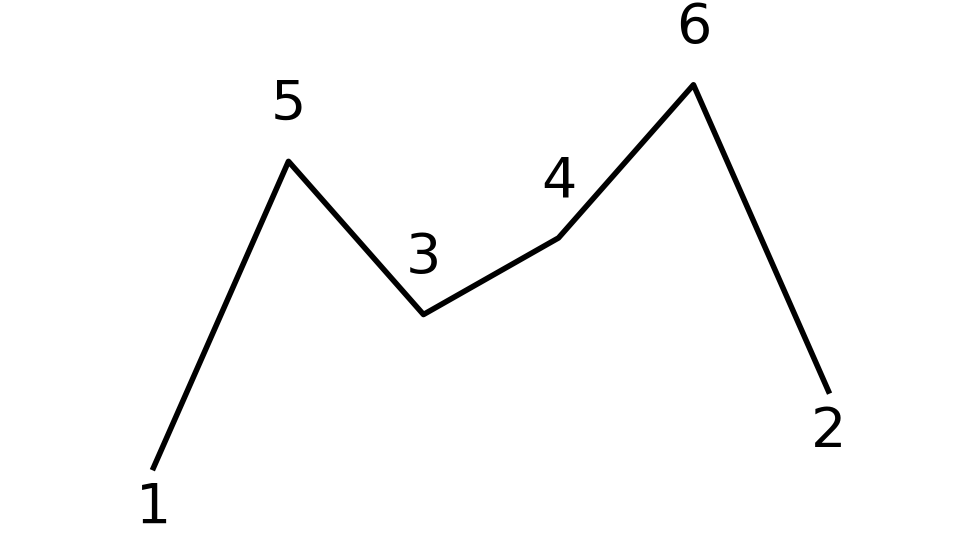
\includegraphics[width=3.5cm]{Introduction/op_P.png} & $T=$ \underline{2 7 4 5 8 3} \underline{1 20 15 16 25 6}  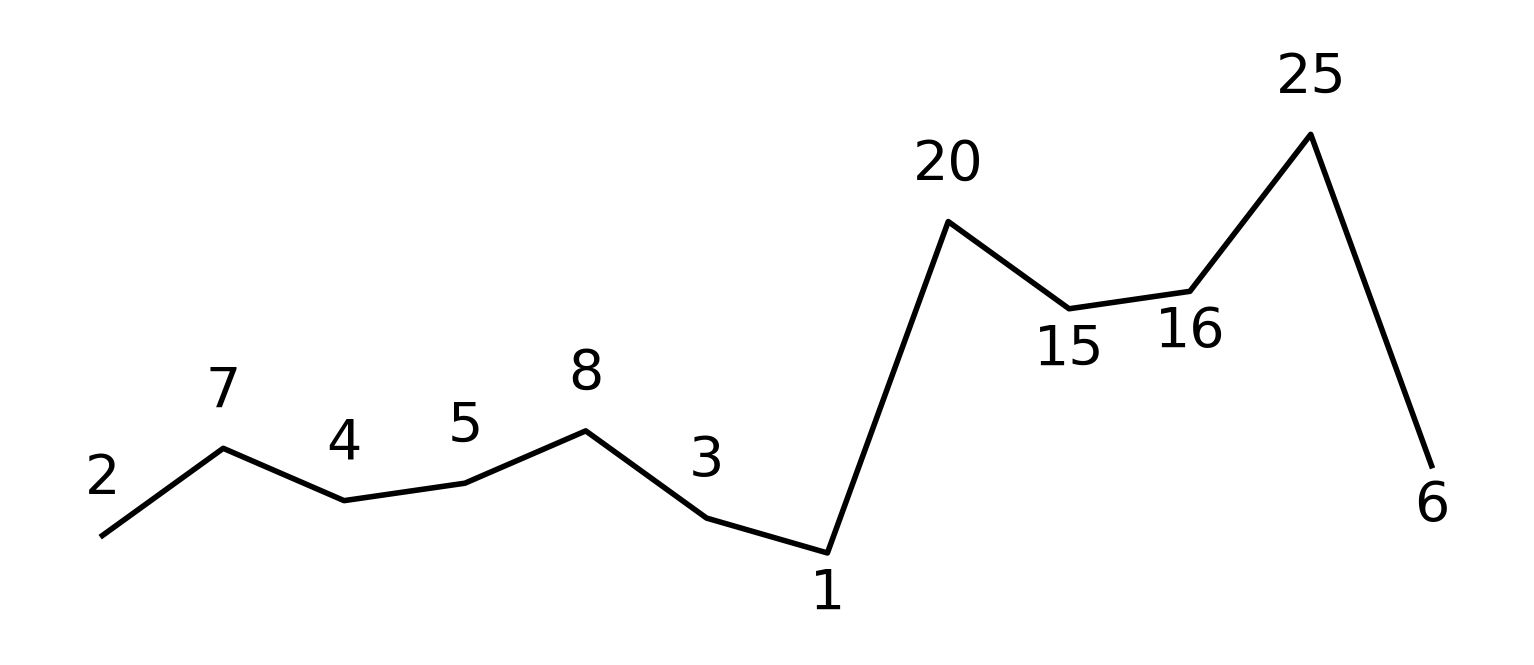
\includegraphics[width=5cm]{Introduction/op_T.png} \\
        %
        Parametrized~\cite{baker1993theory} & $P=$ GATTACAT & $T=$ OPO\underline{POGGODOG}O, {\footnotesize A:O, C:D, G:P, T:G} \\
    \end{tabularx}
    \caption{Example of various model of matching on strings.}
    \label{fig:intro:match_model}
\end{figure}

However, the need for text processing goes far beyond exact pattern matching. To illustrate my point, I give an overview of various text-processing problems and their motivations. Figure~\ref{fig:intro:match_model} also provides an example for each matching model.
% Regular expression
One of the oldest and most classic models for more complex queries is regular expressions introduced by Kleene in 1951~\cite{RM-704}.
% Briefly explain the formalism
This formalism compactly describes a set of strings recursively starting from three operators, concatenation union and Kleene star.
% Application and Limitations
It has deep connections with automatons~\cite{Thompson_automaton}, and its versatile nature makes it a crucial tool in many fields such as internet traffic analysis~\cite{4221791,4579527}, databases, data mining~\cite{1000341,10.5555/645927.672035,10.1145/375551.375569}, computer networks~\cite{10.1145/1159913.1159952}, and protein search~\cite{10.1145/369133.369220}. Chapter~\ref{chap:regexp} provides a new algorithm for Regular expression and pattern matching.

% Similarity measures
Although regular expressions are powerful, Bioinformatics\cite{Gusfield1997}, music analysis~\cite{mongeau1990comparison} and plagiarism detection~\cite{lukashenko2007computer} also need relevant and efficient similarity measures such as the Levenshtein distance~\cite{levenshtein1966binary} or Dynamic Time warping distance~\cite{sakoe1978dynamic}. They also often need to report all occurrences with an error bound\cite{landau1986efficient,landau1989fast}: at a distance at most a threshold $\tau$.
We contribute to this line of research in Chapter~\ref{chap:LCS} and~\ref{chap:DTW}.
% Don't care
As an alternative, Fischer and Paterson~\cite{fischer1974string} introduced "don't care" matching where a don't care symbol denoted * can occur in both the pattern and the text, matches to any other character of the alphabet (but only one).
% Gapped matching
The "don't care" matching model is sometimes referred to as "gapped" matching; however, it is not to be confused with gapped consecutive matching~\cite{bille2022gapped} where we are given two patterns $P_1$ and $P_2$ as well as an interval $[a,b]$ and must report all occurrences of $P_1$ and $P_2$ with the distance in $[a,b]$ and no occurrences in between. This model also has connections to spaced seeds~\cite{burkhardt2003better}, and we study it in Chapter~\ref{chap:gapped_pm} and~\ref{chap:gapped_index}.

% (Elastic) Degenerate strings
The modelization of flexible and diverse DNA sequences~\cite{comm1970iupac} lead to the model of degenerate string~\cite{abrahamson1987generalized} and more recently elastic degenerate strings~\cite{iliopoulos2021efficient}.
% Abelian/jumbled/many other names 
In the model of Abelian matching, a string (or a substring) is entirely identified by the letter it contains (with multiplicities), disregarding their order. It stems from the automatic discovery of clusters of genes in genomes where they can occur in a different order but still linked to the same function~\cite{eres2004permutation}. This model is also known as jumbled, permutation, compomers matching, and many other names, and Tahir Ejaz dedicated his thesis~\cite{ejaz2010abelian} to this model.
% order preserving
The order-preserving model~\cite{kim2014order,kubica2013linear} takes a somewhat opposite approach and considers that two strings match if they have the same relative shape: $\forall i,j \in [0,n-1], X[i] < X[j] \leftrightarrow Y[i] < Y[j]$. This matching model naturally captures the trend detection in the stock market and music melody matching problems.
%
% Parametrized matching
Another application-driven model is parametrized strings or "p-string" introduced by Baker~\cite{baker1993theory}, where two strings match if we can transform one into the other by applying a one-to-tone function renaming the parameters, meant to detect code duplication.\\


% But it is not just about the specific model also about scalibility
We detailed how specific applications can motivate particular string processing tasks, but the scalability in those applications also orient the choice of matching model.

\todo{Example of relevant massive dataset in other area than bioinformatics}

In Bioinformatics, due the cost of next generation sequencing (NGS) has dropped faster than expected by Moore's law~\cite{muir2016real} which led to enormous volume of sequencing data. A quantifiable example of that is the size of the Sequence Read Archive shown in Figure~\ref{fig:intro:sra} since this database tries to capture the major part of the sequencing data produced.

% Why would we need to query the whole archive ?

efficient algorithms and data structures that can leverage the redundant nature of DNA sequences are badly needed. We explore this specific subject in Chapter~\ref{chap:XBWT}

\begin{figure}
    \begin{center}
        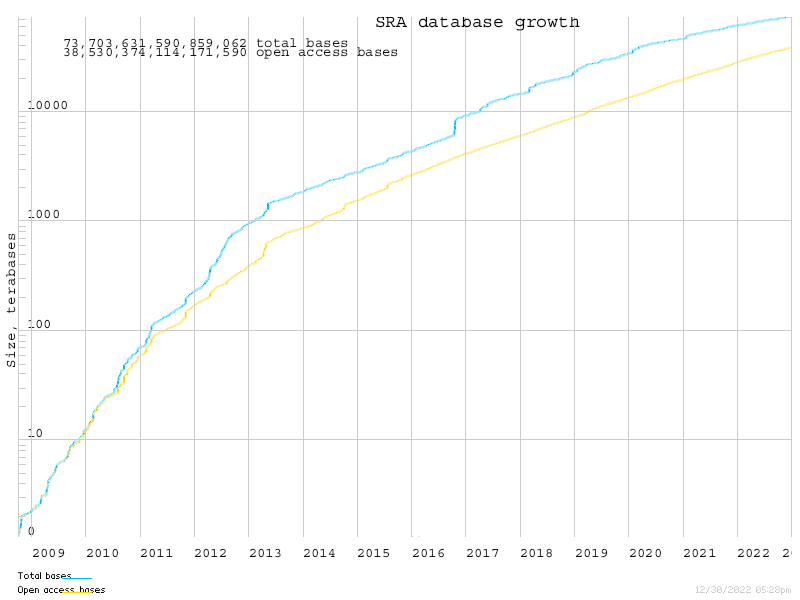
\includegraphics[width=0.8\textwidth]{Introduction/sra_database_growth.png}
        \caption{Evolution of the number of DNA bases in the Sequence Read Archive (SRA), captured from \href{https://www.ncbi.nlm.nih.gov/sra/docs/sragrowth/}{[the dynamic version on the SRA website]}.}
        \label{fig:intro:sra}
    \end{center}
\end{figure}

\todo[inline]{Try to give other example of scalibility issues in other domains}

\subsection*{Approaches to handle massive string data}

\begin{itemize}
\item Data structures and Indexing
\item Streaming algorithm
\item Compressed input
\item Approximation algorithms
\end{itemize}

\begin{itemize}
    \item Detail how we can combine the need for complex queries and scalability
    \item Periodicity
\end{itemize}

\section*{Contributions}

Extend the abstract description of how the different project relate to each other.
